% Options for packages loaded elsewhere
\PassOptionsToPackage{unicode}{hyperref}
\PassOptionsToPackage{hyphens}{url}
%
\documentclass[
]{book}
\usepackage{lmodern}
\usepackage{amssymb,amsmath}
\usepackage{ifxetex,ifluatex}
\ifnum 0\ifxetex 1\fi\ifluatex 1\fi=0 % if pdftex
  \usepackage[T1]{fontenc}
  \usepackage[utf8]{inputenc}
  \usepackage{textcomp} % provide euro and other symbols
\else % if luatex or xetex
  \usepackage{unicode-math}
  \defaultfontfeatures{Scale=MatchLowercase}
  \defaultfontfeatures[\rmfamily]{Ligatures=TeX,Scale=1}
\fi
% Use upquote if available, for straight quotes in verbatim environments
\IfFileExists{upquote.sty}{\usepackage{upquote}}{}
\IfFileExists{microtype.sty}{% use microtype if available
  \usepackage[]{microtype}
  \UseMicrotypeSet[protrusion]{basicmath} % disable protrusion for tt fonts
}{}
\makeatletter
\@ifundefined{KOMAClassName}{% if non-KOMA class
  \IfFileExists{parskip.sty}{%
    \usepackage{parskip}
  }{% else
    \setlength{\parindent}{0pt}
    \setlength{\parskip}{6pt plus 2pt minus 1pt}}
}{% if KOMA class
  \KOMAoptions{parskip=half}}
\makeatother
\usepackage{xcolor}
\IfFileExists{xurl.sty}{\usepackage{xurl}}{} % add URL line breaks if available
\IfFileExists{bookmark.sty}{\usepackage{bookmark}}{\usepackage{hyperref}}
\hypersetup{
  pdftitle={The RJafroc Book},
  pdfauthor={Dev P. Chakraborty, PhD},
  hidelinks,
  pdfcreator={LaTeX via pandoc}}
\urlstyle{same} % disable monospaced font for URLs
\usepackage{color}
\usepackage{fancyvrb}
\newcommand{\VerbBar}{|}
\newcommand{\VERB}{\Verb[commandchars=\\\{\}]}
\DefineVerbatimEnvironment{Highlighting}{Verbatim}{commandchars=\\\{\}}
% Add ',fontsize=\small' for more characters per line
\usepackage{framed}
\definecolor{shadecolor}{RGB}{248,248,248}
\newenvironment{Shaded}{\begin{snugshade}}{\end{snugshade}}
\newcommand{\AlertTok}[1]{\textcolor[rgb]{0.94,0.16,0.16}{#1}}
\newcommand{\AnnotationTok}[1]{\textcolor[rgb]{0.56,0.35,0.01}{\textbf{\textit{#1}}}}
\newcommand{\AttributeTok}[1]{\textcolor[rgb]{0.77,0.63,0.00}{#1}}
\newcommand{\BaseNTok}[1]{\textcolor[rgb]{0.00,0.00,0.81}{#1}}
\newcommand{\BuiltInTok}[1]{#1}
\newcommand{\CharTok}[1]{\textcolor[rgb]{0.31,0.60,0.02}{#1}}
\newcommand{\CommentTok}[1]{\textcolor[rgb]{0.56,0.35,0.01}{\textit{#1}}}
\newcommand{\CommentVarTok}[1]{\textcolor[rgb]{0.56,0.35,0.01}{\textbf{\textit{#1}}}}
\newcommand{\ConstantTok}[1]{\textcolor[rgb]{0.00,0.00,0.00}{#1}}
\newcommand{\ControlFlowTok}[1]{\textcolor[rgb]{0.13,0.29,0.53}{\textbf{#1}}}
\newcommand{\DataTypeTok}[1]{\textcolor[rgb]{0.13,0.29,0.53}{#1}}
\newcommand{\DecValTok}[1]{\textcolor[rgb]{0.00,0.00,0.81}{#1}}
\newcommand{\DocumentationTok}[1]{\textcolor[rgb]{0.56,0.35,0.01}{\textbf{\textit{#1}}}}
\newcommand{\ErrorTok}[1]{\textcolor[rgb]{0.64,0.00,0.00}{\textbf{#1}}}
\newcommand{\ExtensionTok}[1]{#1}
\newcommand{\FloatTok}[1]{\textcolor[rgb]{0.00,0.00,0.81}{#1}}
\newcommand{\FunctionTok}[1]{\textcolor[rgb]{0.00,0.00,0.00}{#1}}
\newcommand{\ImportTok}[1]{#1}
\newcommand{\InformationTok}[1]{\textcolor[rgb]{0.56,0.35,0.01}{\textbf{\textit{#1}}}}
\newcommand{\KeywordTok}[1]{\textcolor[rgb]{0.13,0.29,0.53}{\textbf{#1}}}
\newcommand{\NormalTok}[1]{#1}
\newcommand{\OperatorTok}[1]{\textcolor[rgb]{0.81,0.36,0.00}{\textbf{#1}}}
\newcommand{\OtherTok}[1]{\textcolor[rgb]{0.56,0.35,0.01}{#1}}
\newcommand{\PreprocessorTok}[1]{\textcolor[rgb]{0.56,0.35,0.01}{\textit{#1}}}
\newcommand{\RegionMarkerTok}[1]{#1}
\newcommand{\SpecialCharTok}[1]{\textcolor[rgb]{0.00,0.00,0.00}{#1}}
\newcommand{\SpecialStringTok}[1]{\textcolor[rgb]{0.31,0.60,0.02}{#1}}
\newcommand{\StringTok}[1]{\textcolor[rgb]{0.31,0.60,0.02}{#1}}
\newcommand{\VariableTok}[1]{\textcolor[rgb]{0.00,0.00,0.00}{#1}}
\newcommand{\VerbatimStringTok}[1]{\textcolor[rgb]{0.31,0.60,0.02}{#1}}
\newcommand{\WarningTok}[1]{\textcolor[rgb]{0.56,0.35,0.01}{\textbf{\textit{#1}}}}
\usepackage{longtable,booktabs}
% Correct order of tables after \paragraph or \subparagraph
\usepackage{etoolbox}
\makeatletter
\patchcmd\longtable{\par}{\if@noskipsec\mbox{}\fi\par}{}{}
\makeatother
% Allow footnotes in longtable head/foot
\IfFileExists{footnotehyper.sty}{\usepackage{footnotehyper}}{\usepackage{footnote}}
\makesavenoteenv{longtable}
\usepackage{graphicx}
\makeatletter
\def\maxwidth{\ifdim\Gin@nat@width>\linewidth\linewidth\else\Gin@nat@width\fi}
\def\maxheight{\ifdim\Gin@nat@height>\textheight\textheight\else\Gin@nat@height\fi}
\makeatother
% Scale images if necessary, so that they will not overflow the page
% margins by default, and it is still possible to overwrite the defaults
% using explicit options in \includegraphics[width, height, ...]{}
\setkeys{Gin}{width=\maxwidth,height=\maxheight,keepaspectratio}
% Set default figure placement to htbp
\makeatletter
\def\fps@figure{htbp}
\makeatother
\setlength{\emergencystretch}{3em} % prevent overfull lines
\providecommand{\tightlist}{%
  \setlength{\itemsep}{0pt}\setlength{\parskip}{0pt}}
\setcounter{secnumdepth}{5}
\usepackage{booktabs}
\usepackage{amsthm}
\makeatletter
\def\thm@space@setup{%
  \thm@preskip=8pt plus 2pt minus 4pt
  \thm@postskip=\thm@preskip
}
\makeatother
\usepackage{booktabs}
\usepackage{longtable}
\usepackage{array}
\usepackage{multirow}
\usepackage{wrapfig}
\usepackage{float}
\usepackage{colortbl}
\usepackage{pdflscape}
\usepackage{tabu}
\usepackage{threeparttable}
\usepackage{threeparttablex}
\usepackage[normalem]{ulem}
\usepackage{makecell}
\usepackage{xcolor}
\usepackage[]{natbib}
\bibliographystyle{apalike}

\title{The RJafroc Book}
\author{Dev P. Chakraborty, PhD}
\date{2020-04-27}

\begin{document}
\maketitle

{
\setcounter{tocdepth}{1}
\tableofcontents
}
\hypertarget{preface}{%
\chapter*{Preface}\label{preface}}
\addcontentsline{toc}{chapter}{Preface}

\begin{itemize}
\tightlist
\item
  This book, an extended documentation of the \textbf{RJafroc} package, is currently (as of April 2020) in preperation. It is intended to bypass the file size limits of \textbf{CRAN}, which severely limits the extent of the documentation that can be included with the CRAN package.
\end{itemize}

\hypertarget{a-note-on-the-online-distribution-mechanism-of-the-book}{%
\chapter*{A note on the online distribution mechanism of the book}\label{a-note-on-the-online-distribution-mechanism-of-the-book}}
\addcontentsline{toc}{chapter}{A note on the online distribution mechanism of the book}

\begin{itemize}
\tightlist
\item
  In the hard-copy version of my book \citep{RN2680} the online distribution mechanisms was \texttt{BitBucket}.
\item
  \texttt{BitBucket} allows code sharing within a \emph{closed} group of a few users (e.g., myself and a student).
\item
  Since the purpose of open-source code is to encourage collaborations, this was, in hindsight, an unfortunate choice. Moreover, as my experience with R-packages grew, it became apparent that the vast majority of R-packages are shared on \texttt{GitHub}, not \texttt{BitBucket}.
\item
  For these reasons I have switched to \texttt{GitHub}. Any previous instructions pertaining to \texttt{BitBucket} are obsolete.
\item
  In order to access \texttt{GitHub} material one needs to create a (free) account.
\item
  Go to \href{https://github.com}{this link} and click on \texttt{Sign\ Up}.
\end{itemize}

\hypertarget{contributing-to-this-book}{%
\chapter*{Contributing to this book}\label{contributing-to-this-book}}
\addcontentsline{toc}{chapter}{Contributing to this book}

\begin{itemize}
\tightlist
\item
  I appreciate any feedback on this document, e.g., corrections, comments, etc.\\
\item
  To do this raise an \texttt{Issue} on the \href{https://github.com/dpc10ster/RJafrocBook}{\texttt{GitHub} interface}.
\item
  Click on the \texttt{Issues} tab under \texttt{dpc10ster/RJafrocBook}, then click on \texttt{New\ issue}.
\item
  Contributions from users automatically become part of the \texttt{GitHub} documentation/history of the book.
\end{itemize}

\hypertarget{example-running-external-scripts}{%
\chapter{Example running external scripts}\label{example-running-external-scripts}}

source method

\begin{Shaded}
\begin{Highlighting}[]
\KeywordTok{source}\NormalTok{(}\StringTok{\textquotesingle{}R/example.R\textquotesingle{}}\NormalTok{, }\DataTypeTok{local =}\NormalTok{ T)}
\end{Highlighting}
\end{Shaded}

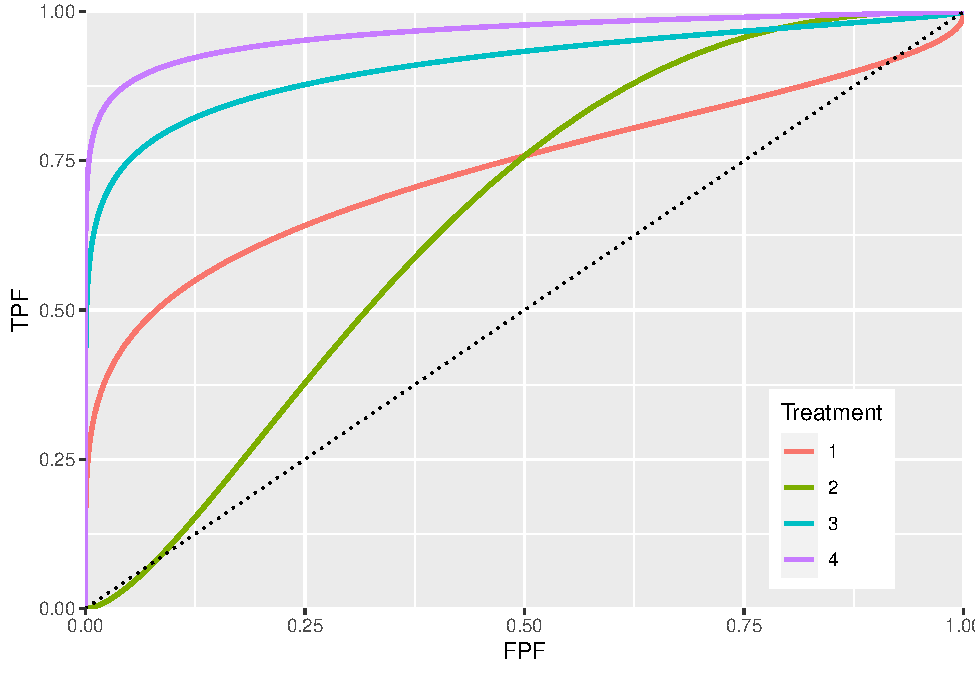
\includegraphics{myReport_files/figure-latex/unnamed-chunk-1-1.pdf}

\begin{Shaded}
\begin{Highlighting}[]
\KeywordTok{print}\NormalTok{(}\KeywordTok{head}\NormalTok{(}\KeywordTok{data.frame}\NormalTok{(x,y)))}
\CommentTok{\#\textgreater{}   x        y}
\CommentTok{\#\textgreater{} 1 1 1.081250}
\CommentTok{\#\textgreater{} 2 2 1.749150}
\CommentTok{\#\textgreater{} 3 3 1.734085}
\CommentTok{\#\textgreater{} 4 4 4.304295}
\CommentTok{\#\textgreater{} 5 5 3.690461}
\CommentTok{\#\textgreater{} 6 6 5.791617}
\end{Highlighting}
\end{Shaded}

read chunk (does not run code)

run the variablesXY chunk and use the variables it creates

\begin{Shaded}
\begin{Highlighting}[]
\NormalTok{x\textless{}{-}}\DecValTok{1}\OperatorTok{:}\DecValTok{100}
\NormalTok{y\textless{}{-}x}\OperatorTok{+}\KeywordTok{rnorm}\NormalTok{(}\DecValTok{100}\NormalTok{)}
\KeywordTok{head}\NormalTok{(}\KeywordTok{data.frame}\NormalTok{(x,y))}
\CommentTok{\#\textgreater{}   x          y}
\CommentTok{\#\textgreater{} 1 1 {-}0.5360904}
\CommentTok{\#\textgreater{} 2 2  1.6600748}
\CommentTok{\#\textgreater{} 3 3  1.9499999}
\CommentTok{\#\textgreater{} 4 4  4.2143395}
\CommentTok{\#\textgreater{} 5 5  4.4061410}
\CommentTok{\#\textgreater{} 6 6  5.8120731}
\end{Highlighting}
\end{Shaded}

run the plotXY chunk and create the plot

\begin{Shaded}
\begin{Highlighting}[]
\KeywordTok{plot}\NormalTok{(x,y)}
\end{Highlighting}
\end{Shaded}

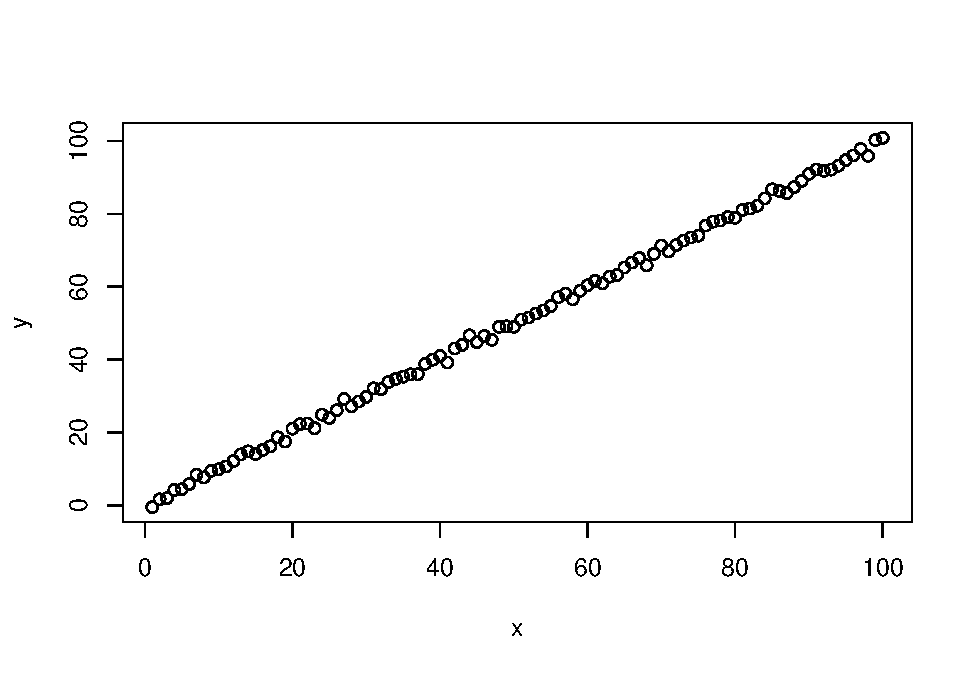
\includegraphics{myReport_files/figure-latex/plotXY-1.pdf}

\hypertarget{ORHAnalysis}{%
\chapter{Obuchowski Rockette Hillis (ORH) Analysis}\label{ORHAnalysis}}

\hypertarget{introduction}{%
\section{Introduction}\label{introduction}}

The previous chapter described the DBM significance testing procedure \citep{RN204} for analyzing MRMC ROC data, along with improvements suggested by Hillis. Because the method assumes that jackknife pseudovalues can be regarded as independent and identically distributed case-level figures of merit, it has been criticized by Hillis who states that the method ``works'' but lacks firm statistical foundations \citep{RN1772, RN1865, RN1866}. If a method works there must be good reasons why it works and the last section of the previous chapter, §9.13, gave a justification for why the method works. Specifically, the empirical AUC pseudovalues qualify as case-level FOMs - this property was also noted by \citep{RN1395}. However, this property applies only to the empirical AUC, so an alternate approach that applies to any figure of merit is desirable.

This chapter presents Hillis' preferred alternative to the DBMH approach. He has argued that the DBMH method can be regarded as a ``working model that gives the right results'', but a method based on an earlier publication \citep{RN1450} by Obuchowski and Rockette, which does not depend on pseudovalues, and predicts more or less the same results, is preferable from a conceptual viewpoint. Since, besides showing the correspondence, Hillis has made significant improvements to the original methodology, this chapter is named ``ORH Analysis'', where ORH stands for Obuchowski, Rockette and Hillis. The ORH method has advantages in being able to handle more complex study designs \citep{RN2508} that are outside the scope of this book (the author acknowledges a private communication from Dr.~Obuchowski, ca. 2006, that demonstrated the flexibility afforded by the OR approach) and it is likely that applications to other FOMs (e.g., the FROC paradigm uses a rather different FOM from empirical ROC-AUC) are better performed with the ORH method.

This chapter starts with a gentle introduction to the Obuchowski and Rockette method. The reason is that the method was rather opaque to me, an I suspect, most users. Part of the problem, in my opinion, is the notation, namely lack of usage of the \emph{case-set} index \(\{c\}\). A key difference of the Obuchowski and Rockette method from DBMH is in how the error term is modeled by a non-diagonal covariance matrix. The structure of the covariance matrix is examined in some detail as it is key to understanding the ORH method.

In the first step of the introduction a single reader interpreting a case-set in multiple treatments is modeled and the results compared to those obtained using DBMH fixed-reader analysis described in the previous chapter. In the second step multiple readers interpreting a case-set in multiple treatments is modeled. The two analyses, DBMH and ORH, are compared for the same dataset. The special cases of fixed-reader and fixed-case analyses are described. Single treatment analysis, where interest is in comparing average performance of readers to a fixed value, is described. Three methods of estimating the covariance matrix are described.

\hypertarget{OR1RMTModel}{%
\section{Single-reader multiple-treatment model}\label{OR1RMTModel}}

Consider a single-reader providing ROC interpretations of a common case-set \(\{c\}\) in multiple-treatments \(i\) (\(i\) = 1, 2, \ldots, \(I\)). Before proceeding, we note that this is not homologous (i.e., formally equivalent) to multiple-readers providing ROC interpretations in a single treatment, §10.7; this is because reader is a random factor while treatment is not. The figure of merit \(\theta\) is modeled as:

\begin{equation}
\theta_{i\{c\}}=\mu+\tau_i+\epsilon_{i\{c\}}
\label{eq:ORModel1RMT}
\end{equation}

\emph{In the \citep{RN1450} one models the figure-of-merit, not the pseudovalues, indeed this is one of the key differences from the DBMH method.}

Recall that \(\{c\}\) denotes a \emph{set of cases}. \eqref{eq:ORModel1RMT} models the observed figure-of-merit \(\theta_{i\{c\}}\) as a constant term \(\mu\) plus a treatment dependent term \(\tau_i\) (the treatment-effect) with the constraint:

\begin{equation}
\sum_{i=1}^{I}\tau_i=0
\label{eq:ConstraintTau}
\end{equation}

The \emph{c-index} was introduced in (book) Chapter 07. The left hand side of \eqref{eq:ORModel1RMT} is the figure-of-merit \(\theta_i\{c\}\) for treatment \(i\) and case-set index \(\{c\}\), where \(c\) = 1, 2, \ldots, \(C\) denotes different independent case-sets sampled from the population, i.e., different collections of \(K_1\) non-diseased and \(K_2\) diseased cases, \emph{not individual cases}.

\emph{This is one place the case-set index is essential for clarity; without it \(\theta_i\) is a fixed quantity - the figure of merit estimate for treatment \(i\) - lacking any index allowing for sampling related variability.}

Obuchowski and Rockette use a \emph{k-index}, defined as the ``kth repetition of the study involving the same diagnostic test, reader and patient (sic)''. In the author's opinion, what is meant is a case-set index instead of a repetition index. Repeating a study with the same treatment, reader and cases yields \emph{within-reader} variability, which is different from sampling the population of cases with new case-sets, which yields \emph{case-sampling plus within-reader} variability. As noted earlier, within-reader variability cannot be ``turned off'' and affects the interpretations of all case-sets.

\emph{Interest is in extrapolating to the population of cases and the only way to do this is to sample different case-sets. It is shown below that usage of the case-set index interpretation yields the same results using the DBMH or the ORH methods.}

Finally, and this is where I had some difficulty understanding what is going on, there is an additive random error term \(\epsilon_{i\{c\}}\) whose sampling behavior is described by a multivariate normal distribution with an I-dimensional zero mean vector and an \(I \times I\) dimensional covariance matrix \(\Sigma\):

\begin{equation}
\epsilon_{i\{c\}} \sim N_I\left ( \vec{0} ,  \Sigma\right )
\label{eq:DefinitionEpsilon}
\end{equation}

Here \(N_I\) is the I-variate normal distribution (i.e., each sample yields \(I\) random numbers). Obuchowski and Rockette assumed the following structure for the covariance matrix (they describe a more general multi-reader model, but here one restricts to the simpler single-reader case):

\begin{equation}
\Sigma_{ii'}=Cov\left ( \epsilon_{i\{c\}}, \epsilon_{i'\{c\}} \right )=\left\{\begin{matrix}
Var \qquad (i=i')\\ 
Cov_1 \qquad (i\neq i')
\end{matrix}\right.
\label{eq:DefinitionSigma}
\end{equation}

The reason for the subscript ``1'' in \(Cov_1\) will become clear when one extends this model to multiple readers. The \(I \times I\) covariance matrix \(\Sigma\) is:

\begin{equation}
\Sigma=
\begin{pmatrix}
Var & Cov_1   & \ldots & Cov_1 & Cov_1 \\
Cov_1 & Var   & \ldots &Cov_1 & Cov_1 \\
\vdots & \vdots & \vdots & \vdots & \vdots \\
Cov_1 & Cov_1 & \ldots & Var & Cov_1 \\
Cov_1 & Cov_1 & \ldots & Cov_1 & Var
\end{pmatrix}
\label{eq:ExampleSigma}
\end{equation}

If \(I\) = 2 then \(\Sigma\) is a symmetric 2 x 2 matrix, whose diagonal terms are the common variances in the two treatments (each assumed equal to \(Var\)) and whose off-diagonal terms (each assumed equal to \(Cov_1\)) are the co-variances. With \(I\) = 3 one has a 3 x 3 symmetric matrix with all diagonal elements equal to \(Var\) and all off-diagonal terms are equal to \(Cov_1\), etc.

\emph{An important aspect of the Obuchowski and Rockette model is that the variances and co-variances are assumed to be treatment independent. This implies that \(Var\) estimates need to be averaged over all treatments. Likewise, \(Cov_1\) estimates need to be averaged over all distinct treatment-treatment pairings.}

A more complex model, with more parameters and therefore more difficult to work with, would allow the variances to be treatment dependent, and the covariances to depend on the specific treatment pairings. For obvious reasons (``Occam's Razor'' or the law of parsimony ) one wishes to start with the simplest model that, one hopes, captures essential characteristics of the data.

Some elementary statistical results are presented next.

\hypertarget{definitions-of-covariance-and-correlation}{%
\subsection{Definitions of covariance and correlation}\label{definitions-of-covariance-and-correlation}}

The covariance of two scalar random variables X and Y is defined by:

\begin{equation}
Cov(X,Y) =\frac{\sum_{i=1}^{N}(x_{i}-x_{\bullet})(y_{i}-y_{\bullet})}{N-1}=E(XY)-E(X)-E(Y)
\label{eq:DefinitionCovariance}
\end{equation}

Here \(E(X)\) is the expectation value of the random variable \(X\), i.e., the integral of x multiplied by its \(pdf\) over the range of \(x\):

\[E(X)=\int pdf(x) x dx\]

The covariance can be thought of as the \emph{common} part of the variance of two random variables. The variance, a special case of covariance, of \(X\) is defined by:

\[Var(X,Y) = Cov(X,X)=E(X^2)-(E(X))^2=\sigma_x^2\]

It can be shown, using the Cauchy--Schwarz inequality, that:

\[\mid Cov(X,Y) \mid^2 \le Var(X)Var(Y)\]

A related quantity, the correlation \(\rho\) is defined by (the \(\sigma\)s are standard deviations):

\[\rho_{XY} \equiv Cor(X,Y)=\frac{Cov(X,Y)}{\sigma_X \sigma_Y}\]

It has the property:

\[\mid \rho_{XY} \mid \le 1\]

\hypertarget{special-case-when-variables-have-equal-variances}{%
\subsection{Special case when variables have equal variances}\label{special-case-when-variables-have-equal-variances}}

Assuming \(X\) and \(Y\) have the same variance:

\[Var(X)=Var(Y)\equiv Var\equiv \sigma^2\]

A useful theorem applicable to the OR single-reader multiple-treatment model is:

\begin{equation}
Var(X-Y)=Var(X)+Var(Y)-2Cov(X,Y)=2(Var-Cov)
\label{eq:UsefulTheorem}
\end{equation}

The first part of the above equation is general, the second part specializes to the OR single-reader multiple-treatment model where the variances are equal and likewise all covariances in \eqref{eq:ExampleSigma} are equal) The correlation \(\rho_1\) is defined by (the reason for the subscript 1 on \(\rho\) is the same as the reason for the subscript 1 on \(Cov_1\), which will be explained later):

\[\rho_1=\frac{Cov_1}{Var}\]

The I x I covariance matrix \(\Sigma\) can be written alternatively as (shown below is the matrix for I = 5; as the matrix is symmetric elements at and above the diagonal are shown):

\begin{equation}
\Sigma = 
\begin{bmatrix}
\sigma^2 & \rho_1\sigma^2 & \rho_1\sigma^2 & \rho_1\sigma^2 & \rho_1\sigma^2\\
& \sigma^2 & \rho_1\sigma^2 & \rho_1\sigma^2 & \rho_1\sigma^2\\
&  & \sigma^2 & \rho_1\sigma^2 & \rho_1\sigma^2\\
&  &  & \sigma^2 & \rho_1\sigma^2\\
&  &  &  & \sigma^2
\end{bmatrix}
\label{eq:ExampleSigmaRho}
\end{equation}

\hypertarget{estimation-of-the-covariance-matrix}{%
\subsection{Estimation of the covariance matrix}\label{estimation-of-the-covariance-matrix}}

An unbiased estimate of the covariance \eqref{eq:DefinitionSigma} follows from:

\begin{equation}
\Sigma_{ii'}=\frac{1}{C-1}\sum_{c=1}^{C} \left ( \theta_{i\{c\}} - \theta_{i\{\bullet\}} \right) \left ( \theta_{i'\{c\}} - \theta_{i'\{\bullet\}} \right)
\label{eq:EstimateSigmaPopulation}
\end{equation}

Sampling different case-sets, as required \eqref{eq:EstimateSigmaPopulation}, is unrealistic and in reality one is stuck with \(C\) = 1, i.e., a single dataset. Therefore, direct application of this formula is impossible. However, as seen when this situation was encountered before in (book) Chapter 07, one can use resampling methods to realize, for example, different bootstrap samples, which are resampling-based ``stand-ins'' for actual case-sets. If \(B\) is the total number of bootstraps, then the estimation formula is:

\begin{equation}
\Sigma_{ii'}\mid_{bs} =\frac{1}{B-1}\sum_{b=1}^{B} \left ( \theta_{i\{b\}} - \theta_{i\{\bullet\}} \right) \left ( \theta_{i'\{b\}} - \theta_{i'\{\bullet\}} \right)
\label{eq:EstimateSigmaBootstrap}
\end{equation}

\eqref{eq:EstimateSigmaBootstrap}, the bootstrap method of estimating the covariance matrix, is a direct translation of \eqref{eq:EstimateSigmaPopulation}. Alternatively, one could have used the jackknife FOM values \(\theta_{i(k)}\), i.e., the figure of merit with a particular case removed, for all cases, to estimate the covariance matrix:

\begin{equation}
\Sigma_{ii'}\mid_{jk} =\frac{(K-1)^2}{K} \left [ \frac{1}{K-1}\sum_{k=1}^{K} \left ( \theta_{i(k)} - \theta_{i(\bullet)} \right) \left ( \theta_{i'(k)} - \theta_{i'(\bullet)} \right) \right ]
\label{eq:EstimateSigmaJackknife}
\end{equation}

Note the subtle difference in notation between \eqref{eq:EstimateSigmaPopulation} and EstimateSigmaJackknife and. In the former, the subscript \(\{c\}\) denotes a set of \(K\) cases while in the latter, \((k)\) denotes the original case set with a particular case \(k\) removed, leaving \(K-1\) cases.

For simplicity, in this section we depart from the usual two-subscript convention to index each case. So \(k\) ranges from 1 to \(K\), where the first \(K_1\) values represent non-diseased and the following \(K_2\) values represent diseased cases. Jackknife figure of merit values are not to be confused with jackknife pseudovalues. The jackknife FOM value corresponding to a particular case is the FOM with the particular case removed. Unlike pseudovalues, jackknife FOM values cannot be regarded as independent and identically distributed. Notice the use of the subscript enclosed in parenthesis \((k)\) to denote the FOM with case \(k\) removed, i.e., a single case, while in the bootstrap equation one uses the curly brackets \(\{b\}\) to denote the bth bootstrap \emph{case-set}, i.e., a whole set of \(K_1\) non-diseased and \(K_2\) diseased cases, sampled with replacement from the original dataset. Furthermore, the expression for the jackknife covariance contains a \emph{variance inflation factor}:

\begin{equation}
\frac{(K-1)^2}{K}
\label{eq:JKVarianceInflationFactor}
\end{equation}

This factor multiplies the traditional expression for the covariance, shown in square brackets in \eqref{eq:EstimateSigmaJackknife}. A third method of estimating the covariance, namely the DeLong et al.~method \citep{RN112}, applicable only to the empirical AUC, is described later.

\hypertarget{meaning-of-the-covariance-matrix-in-refeqexamplesigma}{%
\subsection{Meaning of the covariance matrix in \eqref{eq:ExampleSigma}}\label{meaning-of-the-covariance-matrix-in-refeqexamplesigma}}

Suppose one has the luxury of repeatedly sampling case-sets, each consisting of \(K\) cases from the population. A single radiologist interprets these cases in \(I\) treatments. Therefore, each case-set \(\{c\}\) yields \(I\) figures of merit. The final numbers at ones disposal are \(\theta_{i\{c\}}\), where \(i\) = 1,2,\ldots,\(I\) and \(c\) = 1,2,\ldots,\(C\). Considering treatment \(i\), the variance of the FOM-values for the different case-sets \(c\) = 1,2,\ldots,\(C\), is an estimate of \(Var_i\) for this treatment:

\begin{equation}
\sigma_i^2 \equiv Var_i = \frac{1}{C-1}\sum_{c=1}^{C}\left ( \theta_{i\{c\}} - \theta_{i\{\bullet\}} \right) \left ( \theta_{i\{c\}} - \theta_{i\{\bullet\}} \right)
\label{eq:EstimateVari}
\end{equation}

The process is repeated for all treatments and the \(I\)-variance values are averaged. This is the final estimate of \(Var\) appearing in \eqref{eq:DefinitionEpsilon}.

To estimate the covariance matrix one considers pairs of FOM values for the same case-set \(\{c\}\) but different treatments, i.e., \(\theta_{i\{c\}}\) and \(\theta_{i'\{c\}}\); \emph{by definition primed and un-primed indices are different}. Since they are derived from the same case-set, one expects the values to be correlated. For a particularly easy case-set one expects all I-estimates to be collectively higher than usual. The process is repeated for different case-sets and one calculates the correlation \(\rho_{1;ii'}\) between the two \(C\)-length arrays \(\theta_{i\{c\}}\) and \(\theta_{i'\{c\}}\):

\begin{equation}
\rho_{1;ii'} = \frac{1}{C-1}\sum_{c=1}^{C} \frac {\left ( \theta_{i\{c\}} - \theta_{i\{\bullet\}} \right) \left ( \theta_{i'\{c\}} - \theta_{i'\{\bullet\}} \right)}{\sigma_i \sigma_{i'} }
\label{eq:EstimateRho}
\end{equation}

The entire process is repeated for different treatment pairings and the resulting \(I(I-1)/2\) distinct values are averaged yielding the final estimate of \(\rho_1\) in \eqref{eq:ExampleSigmaRho}. According to @ref(eq: EstimateRho) one expects the covariance to be smaller than the variance determined as in the previous paragraph.

In most situations one expects \(\rho_1\) (for ROC studies) to be positive. There is, perhaps unlikely, a scenario that could lead to anti-correlation and negative. This could occur, with ``complementary'' treatments, e.g., CT vs.~MRI, where one treatment is good for bone imaging and the other for soft-tissue imaging. In this situation what constitutes an easy case-set in one treatment could be a difficult case-set in the other treatment.

\hypertarget{code-illustrating-the-covariance-matrix-tba}{%
\subsection{Code illustrating the covariance matrix (TBA)}\label{code-illustrating-the-covariance-matrix-tba}}

As indicated above, the covariance matrix can be estimated using the jackknife or the bootstrap. If the figure of merit is the Wilcoxon statistic, then one can also use the DeLong et al method \citep{RN112}. In (book) Chapter 07, these methods were described in the context of estimating the variance of AUC. \eqref{eq:EstimateSigmaBootstrap} and \eqref{eq:EstimateSigmaJackknife} extend the jackknife and the bootstrap methods, respectively, to estimating the covariance of AUC (whose diagonal elements are the variances estimated in the earlier chapter). The extension of the DeLong method to covariances is described in Online Appendix 10.A (TBA) and implemented in file \texttt{VarCovMtrxDLStr.R}. The implementation of the DeLong method \citep{RN112} in file \texttt{VarCovMtrxDLStr.R} gives identical results to those yielded by the SAS macro attributed to DeLong. The file name stands for ``variance covariance matrix according to the DeLong structural components method'' \emph{described in five unnumbered equations following Eqn. 4 in the cited reference}.

The jackknife, bootstrap and the DeLong methods are used in file \texttt{mainVarCov1.R}, a listing and explanation of which appears in (TBA) Online Appendix 10.B. Source the file yielding the following code output:

\begin{itemize}
\item
  The codes for the functions (for \texttt{Var} and \texttt{Cov1} using bootstrap, jackknife, and the DeLong methods) are not displayed (but they are compiled). To display them download the repository and look at the corresponding \texttt{Rmd} file.
\item
  Here is the code to calculate the Wilcoxon statistic.
\item
  Here is the code to calculate \texttt{Cov1} and \texttt{Var} using the bootstrap method.
\item
  Here is the code to calculate \texttt{Cov1} and \texttt{Var} using the jackknife method.
\item
  Here is the code to calculate \texttt{Cov1} and \texttt{Var} using the DeLong method.
\end{itemize}

The following code uses the functions defined above to calculate \texttt{Cov1} and \texttt{Var} different ways.

\begin{Shaded}
\begin{Highlighting}[]
\NormalTok{seed \textless{}{-}}\StringTok{ }\DecValTok{1}\NormalTok{;}\KeywordTok{set.seed}\NormalTok{(seed)}
\CommentTok{\#select the 1st reader to be analyzed}
\NormalTok{rocData1R \textless{}{-}}\StringTok{ }\KeywordTok{DfExtractDataset}\NormalTok{(dataset02, }\DataTypeTok{rdrs =} \DecValTok{1}\NormalTok{)}

\NormalTok{zik1 \textless{}{-}}\StringTok{ }\NormalTok{rocData1R}\OperatorTok{$}\NormalTok{NL[,}\DecValTok{1}\NormalTok{,,}\DecValTok{1}\NormalTok{];K \textless{}{-}}\StringTok{ }\KeywordTok{dim}\NormalTok{(zik1)[}\DecValTok{2}\NormalTok{];I \textless{}{-}}\StringTok{ }\KeywordTok{dim}\NormalTok{(zik1)[}\DecValTok{1}\NormalTok{]}
\NormalTok{zik2 \textless{}{-}}\StringTok{ }\NormalTok{rocData1R}\OperatorTok{$}\NormalTok{LL[,}\DecValTok{1}\NormalTok{,,}\DecValTok{1}\NormalTok{];K2 \textless{}{-}}\StringTok{ }\KeywordTok{dim}\NormalTok{(zik2)[}\DecValTok{2}\NormalTok{];K1 \textless{}{-}}\StringTok{ }\NormalTok{K}\OperatorTok{{-}}\NormalTok{K2;zik1 \textless{}{-}}\StringTok{ }\NormalTok{zik1[,}\DecValTok{1}\OperatorTok{:}\NormalTok{K1]}

\CommentTok{\# jk = jackknife}
\CommentTok{\# rjjk = RJafroc, covEstMethod = "jackknife"}
\CommentTok{\# rjbs = RJafroc, covEstMethod = "bootstrap"}
\CommentTok{\# bs = bootstrap}
\CommentTok{\# dl = DeLong}
\NormalTok{ret1 \textless{}{-}}\StringTok{ }\KeywordTok{VarCov1\_Jk}\NormalTok{(zik1, zik2)}
\NormalTok{Var \textless{}{-}}\StringTok{ }\NormalTok{ret1}\OperatorTok{$}\NormalTok{Var;Cov1 \textless{}{-}}\StringTok{ }\NormalTok{ret1}\OperatorTok{$}\NormalTok{Cov1 }\CommentTok{\# use these (i.e., jackknife) as default values in subsequent code}
\KeywordTok{data.frame}\NormalTok{ (}\StringTok{"Cov\_jk"}\NormalTok{ =}\StringTok{ }\NormalTok{Cov1, }\StringTok{"Var\_jk"}\NormalTok{ =}\StringTok{ }\NormalTok{Var)}
\CommentTok{\#\textgreater{}         Cov\_jk       Var\_jk}
\CommentTok{\#\textgreater{} 1 0.0003734661 0.0006989006}

\NormalTok{ret4 \textless{}{-}}\StringTok{ }\KeywordTok{UtilVarComponentsOR}\NormalTok{(rocData1R, }\DataTypeTok{FOM =} \StringTok{"Wilcoxon"}\NormalTok{)}\OperatorTok{$}\NormalTok{varComp}
\KeywordTok{data.frame}\NormalTok{ (}\StringTok{"Cov\_rjjk"}\NormalTok{ =}\StringTok{ }\NormalTok{ret4}\OperatorTok{$}\NormalTok{cov1, }\StringTok{"Var\_rjjk"}\NormalTok{ =}\StringTok{ }\NormalTok{ret4}\OperatorTok{$}\NormalTok{var)}
\CommentTok{\#\textgreater{}       Cov\_rjjk     Var\_rjjk}
\CommentTok{\#\textgreater{} 1 0.0003734661 0.0006989006}

\NormalTok{ret2 \textless{}{-}}\StringTok{ }\KeywordTok{VarCov1\_Bs}\NormalTok{(zik1, zik2, }\DecValTok{2000}\NormalTok{) }\CommentTok{\# 2000 bootstraps}
\KeywordTok{data.frame}\NormalTok{ (}\StringTok{"Cov\_bs"}\NormalTok{ =}\StringTok{ }\NormalTok{ret2}\OperatorTok{$}\NormalTok{Cov1, }\StringTok{"Var\_bs"}\NormalTok{ =}\StringTok{ }\NormalTok{ret2}\OperatorTok{$}\NormalTok{Var) }
\CommentTok{\#\textgreater{}         Cov\_bs       Var\_bs}
\CommentTok{\#\textgreater{} 1 0.0003466804 0.0006738506}

\NormalTok{ret5 \textless{}{-}}\StringTok{ }\KeywordTok{UtilVarComponentsOR}\NormalTok{(rocData1R, }\DataTypeTok{FOM =} \StringTok{"Wilcoxon"}\NormalTok{, }\DataTypeTok{covEstMethod =} \StringTok{"bootstrap"}\NormalTok{, }\DataTypeTok{nBoots =} \DecValTok{200}\NormalTok{)}\OperatorTok{$}\NormalTok{varComp}
\KeywordTok{data.frame}\NormalTok{ (}\StringTok{"Cov\_rjbs"}\NormalTok{ =}\StringTok{ }\NormalTok{ret5}\OperatorTok{$}\NormalTok{cov1, }\StringTok{"Var\_rjbs"}\NormalTok{ =}\StringTok{ }\NormalTok{ret5}\OperatorTok{$}\NormalTok{var)}
\CommentTok{\#\textgreater{}      Cov\_rjbs     Var\_rjbs}
\CommentTok{\#\textgreater{} 1 0.000283905 0.0005845354}

\NormalTok{ret5 \textless{}{-}}\StringTok{ }\KeywordTok{UtilVarComponentsOR}\NormalTok{(rocData1R, }\DataTypeTok{FOM =} \StringTok{"Wilcoxon"}\NormalTok{, }\DataTypeTok{covEstMethod =} \StringTok{"bootstrap"}\NormalTok{, }\DataTypeTok{nBoots =} \DecValTok{2000}\NormalTok{)}\OperatorTok{$}\NormalTok{varComp}
\KeywordTok{data.frame}\NormalTok{ (}\StringTok{"Cov\_rjbs"}\NormalTok{ =}\StringTok{ }\NormalTok{ret5}\OperatorTok{$}\NormalTok{cov1, }\StringTok{"Var\_rjbs"}\NormalTok{ =}\StringTok{ }\NormalTok{ret5}\OperatorTok{$}\NormalTok{var) }\CommentTok{\# matches local code with 2000 nBoots, provided seeds are identical}
\CommentTok{\#\textgreater{}       Cov\_rjbs     Var\_rjbs}
\CommentTok{\#\textgreater{} 1 0.0003466804 0.0006738506}

\NormalTok{ret5 \textless{}{-}}\StringTok{ }\KeywordTok{UtilVarComponentsOR}\NormalTok{(rocData1R, }\DataTypeTok{FOM =} \StringTok{"Wilcoxon"}\NormalTok{, }\DataTypeTok{covEstMethod =} \StringTok{"bootstrap"}\NormalTok{, }\DataTypeTok{nBoots =} \DecValTok{20000}\NormalTok{)}\OperatorTok{$}\NormalTok{varComp}
\KeywordTok{data.frame}\NormalTok{ (}\StringTok{"Cov\_rjbs"}\NormalTok{ =}\StringTok{ }\NormalTok{ret5}\OperatorTok{$}\NormalTok{cov1, }\StringTok{"Var\_rjbs"}\NormalTok{ =}\StringTok{ }\NormalTok{ret5}\OperatorTok{$}\NormalTok{var)}
\CommentTok{\#\textgreater{}       Cov\_rjbs     Var\_rjbs}
\CommentTok{\#\textgreater{} 1 0.0003680714 0.0006862668}

\NormalTok{mtrxDLStr \textless{}{-}}\StringTok{ }\KeywordTok{VarCovMtrxDLStr}\NormalTok{(rocData1R)}
\NormalTok{ret3 \textless{}{-}}\StringTok{ }\KeywordTok{VarCovs}\NormalTok{(mtrxDLStr)}

\KeywordTok{data.frame}\NormalTok{ (}\StringTok{"Cov\_dl"}\NormalTok{ =}\StringTok{ }\NormalTok{ret3}\OperatorTok{$}\NormalTok{cov1, }\StringTok{"Var\_dl"}\NormalTok{ =}\StringTok{ }\NormalTok{ret3}\OperatorTok{$}\NormalTok{var)}
\CommentTok{\#\textgreater{}         Cov\_dl       Var\_dl}
\CommentTok{\#\textgreater{} 1 0.0003684357 0.0006900766}
\end{Highlighting}
\end{Shaded}

\hypertarget{tba-discussion-of-above-code}{%
\subsection{TBA Discussion of above code}\label{tba-discussion-of-above-code}}

\hypertarget{significance-testing}{%
\subsection{Significance testing}\label{significance-testing}}

The covariance matrix is needed for significance testing. Define the mean square corresponding to the treatment effect, denoted \(MS(T)\), by:

\begin{equation}
MS(T)=\frac{1}{I-1}\sum_{i=1}^{I}(\theta_i-\theta_\bullet)^2
\label{eq:DefinitionMST}
\end{equation}

\emph{Unlike the previous chapter, all mean square quantities defined in this chapter are based on FOMs, not pseudovalues.}

It can be shown that under the null hypothesis (that all treatments have identical performances) the test statistic \(\chi_{1R}\) defined below (the \(1R\) subscript denotes single-reader analysis) is distributed approximately as a \(\chi^2\) distribution with \(I-1\) degrees of freedom, i.e.,

\begin{equation}
\chi_{1R} \equiv \frac{(I-1)MS(T)}{Var-Cov_1} \sim \chi_{I-1}^{2}
\label{eq:F-1RMT}
\end{equation}

\eqref{eq:F-1RMT} is from §5.4 \citep{RN1865} with two covariance terms ``zeroed out'' because they are multiplied by \(J-1 = 0\) (since, in this example, we are restricting to \(J=1\)).

Or equivalently, in terms of the F-distribution \citep{RN1772}:

\begin{equation}
F_{1R} \equiv \frac{MS(T)}{Var-Cov_1} \sim F_{I-1, \infty}
\label{eq:DefF-1RMT}
\end{equation}

\hypertarget{an-aside-on-the-relation-between-the-chisquare-and-the-f-distribution-with-infinite-ddf}{%
\subsubsection{An aside on the relation between the chisquare and the F-distribution with infinite ddf}\label{an-aside-on-the-relation-between-the-chisquare-and-the-f-distribution-with-infinite-ddf}}

Define \(D_{1-\alpha}\), the \((1-\alpha)\) quantile of distribution \(D\), as that ``cutoff'' value such that the probability of observing a random sample \(d\) less than or equal to \(D_{1-\alpha}\) is \((1-\alpha)\). In other words,

\begin{equation}
\Pr(d\leq D_{1-alpha} \mid d \sim D)=1-\alpha
\label{eq:DefQuantile}
\end{equation}

With definition \eqref{eq:DefQuantile}, the \((1-\alpha)\) quantile of the \(\chi_{I-1}^2\) distribution, i.e., \(\chi_{1-\alpha,I-1}^2\), is related to the \((1-\alpha)\) quantile of the \(F_{I-1,\infty}\) distribution, i.e., \(F_{1-\alpha,I-1,\infty}\), as follows \citep[see][Eq. 22]{RN1772}:

\begin{equation}
\frac{\chi_{1-\alpha,I-1}^{2}}{I-1} = F_{1-\alpha,I-1,\infty}
\label{eq:Chisqr2F}
\end{equation}

\eqref{eq:Chisqr2F} implies that the \((1-\alpha)\) quantile of the F-distribution with \(ndf=(I-1)\) and \(ddf=\infty\) equals the \((1-\alpha)\) quantile of the \(\chi_{I-1}^2\) distribution \emph{divided by \((I-1)\)}.

Here is an \texttt{R} illustration of this theorem for \(I-1 = 4\) and \(\alpha = 0.05\):

\begin{Shaded}
\begin{Highlighting}[]
\KeywordTok{qf}\NormalTok{(}\FloatTok{0.05}\NormalTok{, }\DecValTok{4}\NormalTok{, }\OtherTok{Inf}\NormalTok{)}
\CommentTok{\#\textgreater{} [1] 0.1776808}
\KeywordTok{qchisq}\NormalTok{(}\FloatTok{0.05}\NormalTok{,}\DecValTok{4}\NormalTok{)}\OperatorTok{/}\DecValTok{4}
\CommentTok{\#\textgreater{} [1] 0.1776808}
\end{Highlighting}
\end{Shaded}

\hypertarget{p-value-and-confidence-interval}{%
\subsection{p-value and confidence interval}\label{p-value-and-confidence-interval}}

The p-value is the probability that a sample from the \(F_{I-1,\infty}\) distribution is greater than or equal to the observed value of the test statistic, namely:

\begin{equation}
p\equiv \Pr(f>F_{1R} \mid f \sim F_{I-1,\infty})
\label{eq:pValue1RMT}
\end{equation}

The \((1-\alpha)\) confidence interval for the inter-treatment FOM difference is given by:

\begin{equation}
CI_{1-\alpha,1RMT} = (\theta_{i\bullet} - \theta_{i'\bullet}) \pm t_{\alpha/2,\infty} \sqrt{2(Var-Cov_1)}
\label{eq:CIalpha1RMT}
\end{equation}

Comparing \eqref{eq:CIalpha1RMT} to \eqref{eq:UsefulTheorem} shows that the term \(\sqrt{2(Var-Cov_1)}\) is the standard error of the inter-treatment FOM difference, whose square root is the standard deviation. The term \(t_{\alpha/2,\infty}\) is -1.96 and \(t_{1-\alpha/2,\infty}\) is +1.96. Therefore, the confidence interval is constructed by adding and subtracting 1.96 times the standard deviation of the difference from the central value. {[}One has probably encountered the rule that a 95\% confidence interval is plus or minus two standard deviations from the central value. The ``2'' comes from rounding up 1.96.{]}

\hypertarget{comparing-dbm-to-obuchowski-and-rockette-for-single-reader-multiple-treatments}{%
\subsection{Comparing DBM to Obuchowski and Rockette for single-reader multiple-treatments}\label{comparing-dbm-to-obuchowski-and-rockette-for-single-reader-multiple-treatments}}

We have shown two methods for analyzing a single reader in multiple treatments: the DBMH method, involving jackknife derived pseudovalues and the Obuchowski and Rockette method that does not have to use the jackknife, since it could use the bootstrap to get the covariance matrix, or some other methods such as the DeLong method, if one restricts to the Wilcoxon statistic for the figure of merit (empirical ROC-AUC). Since one is dealing with a single reader in multiple treatments, for DBMH one needs the fixed-reader analysis described in §9.8 the previous chapter (with one reader the conclusions obviousl apply to the specific reader, so reader must be regarded as a fixed factor). Source the file (TBA) MainOrDbmh1R.R, a listing of which appears in (TBA) Online Appendix 10.C. For convenience, a few relevant lines are shown here:

\begin{Shaded}
\begin{Highlighting}[]
\CommentTok{\# seed \textless{}{-} 1;set.seed(seed)}
\NormalTok{alpha \textless{}{-}}\StringTok{ }\FloatTok{0.05}
\NormalTok{theta\_i \textless{}{-}}\StringTok{ }\KeywordTok{c}\NormalTok{(}\DecValTok{0}\NormalTok{,}\DecValTok{0}\NormalTok{);}\ControlFlowTok{for}\NormalTok{ (i }\ControlFlowTok{in} \DecValTok{1}\OperatorTok{:}\NormalTok{I) theta\_i[i] \textless{}{-}}\StringTok{ }\KeywordTok{Wilcoxon}\NormalTok{(zik1[i,], zik2[i,])}

\NormalTok{MS\_T \textless{}{-}}\StringTok{ }\DecValTok{0}
\ControlFlowTok{for}\NormalTok{ (i }\ControlFlowTok{in} \DecValTok{1}\OperatorTok{:}\NormalTok{I) \{}
\NormalTok{  MS\_T \textless{}{-}}\StringTok{ }\NormalTok{MS\_T }\OperatorTok{+}\StringTok{ }\NormalTok{(theta\_i[i]}\OperatorTok{{-}}\KeywordTok{mean}\NormalTok{(theta\_i))}\OperatorTok{\^{}}\DecValTok{2}
\NormalTok{\}}
\NormalTok{MS\_T \textless{}{-}}\StringTok{ }\NormalTok{MS\_T}\OperatorTok{/}\NormalTok{(I}\DecValTok{{-}1}\NormalTok{)}

\NormalTok{F\_1R \textless{}{-}}\StringTok{ }\NormalTok{MS\_T}\OperatorTok{/}\NormalTok{(Var }\OperatorTok{{-}}\StringTok{ }\NormalTok{Cov1)}
\NormalTok{pValue \textless{}{-}}\StringTok{ }\DecValTok{1} \OperatorTok{{-}}\StringTok{ }\KeywordTok{pf}\NormalTok{(F\_1R, I}\DecValTok{{-}1}\NormalTok{, }\OtherTok{Inf}\NormalTok{)}

\NormalTok{trtDiff \textless{}{-}}\StringTok{ }\KeywordTok{array}\NormalTok{(}\DataTypeTok{dim =} \KeywordTok{c}\NormalTok{(I,I))}
\ControlFlowTok{for}\NormalTok{ (i1 }\ControlFlowTok{in} \DecValTok{1}\OperatorTok{:}\NormalTok{(I}\DecValTok{{-}1}\NormalTok{)) \{    }
  \ControlFlowTok{for}\NormalTok{ (i2 }\ControlFlowTok{in}\NormalTok{ (i1}\OperatorTok{+}\DecValTok{1}\NormalTok{)}\OperatorTok{:}\NormalTok{I) \{}
\NormalTok{    trtDiff[i1,i2] \textless{}{-}}\StringTok{ }\NormalTok{theta\_i[i1]}\OperatorTok{{-}}\StringTok{ }\NormalTok{theta\_i[i2]    }
\NormalTok{  \}}
\NormalTok{\}}
\NormalTok{trtDiff \textless{}{-}}\StringTok{ }\NormalTok{trtDiff[}\OperatorTok{!}\KeywordTok{is.na}\NormalTok{(trtDiff)]}
\NormalTok{nDiffs \textless{}{-}}\StringTok{ }\NormalTok{I}\OperatorTok{*}\NormalTok{(I}\DecValTok{{-}1}\NormalTok{)}\OperatorTok{/}\DecValTok{2}
\NormalTok{CI\_DIFF\_FOM\_1RMT \textless{}{-}}\StringTok{ }\KeywordTok{array}\NormalTok{(}\DataTypeTok{dim =} \KeywordTok{c}\NormalTok{(nDiffs, }\DecValTok{3}\NormalTok{))}
\ControlFlowTok{for}\NormalTok{ (i }\ControlFlowTok{in} \DecValTok{1} \OperatorTok{:}\StringTok{ }\NormalTok{nDiffs) \{}
\NormalTok{  CI\_DIFF\_FOM\_1RMT[i,}\DecValTok{1}\NormalTok{] \textless{}{-}}\StringTok{ }\KeywordTok{qt}\NormalTok{(alpha}\OperatorTok{/}\DecValTok{2}\NormalTok{,}\DataTypeTok{df =} \OtherTok{Inf}\NormalTok{)}\OperatorTok{*}\KeywordTok{sqrt}\NormalTok{(}\DecValTok{2}\OperatorTok{*}\NormalTok{(Var }\OperatorTok{{-}}\StringTok{ }\NormalTok{Cov1)) }\OperatorTok{+}\StringTok{ }\NormalTok{trtDiff[i]}
\NormalTok{  CI\_DIFF\_FOM\_1RMT[i,}\DecValTok{2}\NormalTok{] \textless{}{-}}\StringTok{ }\NormalTok{trtDiff[i]}
\NormalTok{  CI\_DIFF\_FOM\_1RMT[i,}\DecValTok{3}\NormalTok{] \textless{}{-}}\StringTok{ }\KeywordTok{qt}\NormalTok{(}\DecValTok{1}\OperatorTok{{-}}\NormalTok{alpha}\OperatorTok{/}\DecValTok{2}\NormalTok{,}\DataTypeTok{df =} \OtherTok{Inf}\NormalTok{)}\OperatorTok{*}\KeywordTok{sqrt}\NormalTok{(}\DecValTok{2}\OperatorTok{*}\NormalTok{(Var }\OperatorTok{{-}}\StringTok{ }\NormalTok{Cov1)) }\OperatorTok{+}\StringTok{ }\NormalTok{trtDiff[i]}
  \KeywordTok{print}\NormalTok{(}\KeywordTok{data.frame}\NormalTok{(}\StringTok{"theta\_1"}\NormalTok{ =}\StringTok{ }\NormalTok{theta\_i[}\DecValTok{1}\NormalTok{],}
                   \StringTok{"theta\_2"}\NormalTok{ =}\StringTok{ }\NormalTok{theta\_i[}\DecValTok{2}\NormalTok{],}
                   \StringTok{"Var"}\NormalTok{ =}\StringTok{ }\NormalTok{Var,}
                   \StringTok{"Cov1"}\NormalTok{ =}\StringTok{ }\NormalTok{Cov1,}
                   \StringTok{"MS\_T"}\NormalTok{ =}\StringTok{ }\NormalTok{MS\_T,}
                   \StringTok{"F\_1R"}\NormalTok{ =}\StringTok{ }\NormalTok{F\_1R, }
                   \StringTok{"pValue"}\NormalTok{ =}\StringTok{ }\NormalTok{pValue,}
                   \StringTok{"Lower"}\NormalTok{ =}\StringTok{ }\NormalTok{CI\_DIFF\_FOM\_1RMT[i,}\DecValTok{1}\NormalTok{], }
                   \StringTok{"Mid"}\NormalTok{ =}\StringTok{ }\NormalTok{CI\_DIFF\_FOM\_1RMT[i,}\DecValTok{2}\NormalTok{], }
                   \StringTok{"Upper"}\NormalTok{ =}\StringTok{ }\NormalTok{CI\_DIFF\_FOM\_1RMT[i,}\DecValTok{3}\NormalTok{]))}
\NormalTok{\}}
\CommentTok{\#\textgreater{}     theta\_1   theta\_2          Var         Cov1         MS\_T     F\_1R    pValue}
\CommentTok{\#\textgreater{} 1 0.9196457 0.9478261 0.0006989006 0.0003734661 0.0003970662 1.220111 0.2693389}
\CommentTok{\#\textgreater{}         Lower         Mid      Upper}
\CommentTok{\#\textgreater{} 1 {-}0.07818322 {-}0.02818035 0.02182251}
\CommentTok{\# compare to RJafroc}
\NormalTok{ret\_rj \textless{}{-}}\StringTok{ }\KeywordTok{StSignificanceTesting}\NormalTok{(rocData1R, }\DataTypeTok{FOM =} \StringTok{"Wilcoxon"}\NormalTok{, }\DataTypeTok{method =} \StringTok{"ORH"}\NormalTok{)}
\KeywordTok{print}\NormalTok{(}\KeywordTok{data.frame}\NormalTok{(}\StringTok{"theta\_1"}\NormalTok{ =}\StringTok{ }\NormalTok{ret\_rj}\OperatorTok{$}\NormalTok{fomArray[}\DecValTok{1}\NormalTok{],}
                 \StringTok{"theta\_2"}\NormalTok{ =}\StringTok{ }\NormalTok{ret\_rj}\OperatorTok{$}\NormalTok{fomArray[}\DecValTok{2}\NormalTok{],}
                 \StringTok{"Var"}\NormalTok{ =}\StringTok{ }\NormalTok{ret\_rj}\OperatorTok{$}\NormalTok{varComp}\OperatorTok{$}\NormalTok{var,}
                 \StringTok{"Cov1"}\NormalTok{ =}\StringTok{ }\NormalTok{ret\_rj}\OperatorTok{$}\NormalTok{varComp}\OperatorTok{$}\NormalTok{cov,}
                 \StringTok{"MS\_T"}\NormalTok{ =}\StringTok{ }\NormalTok{ret\_rj}\OperatorTok{$}\NormalTok{msT,}
                 \StringTok{"F\_1R"}\NormalTok{ =}\StringTok{ }\NormalTok{ret\_rj}\OperatorTok{$}\NormalTok{FTestStatsFRRC}\OperatorTok{$}\NormalTok{fFRRC, }
                 \StringTok{"pValue"}\NormalTok{ =}\StringTok{ }\NormalTok{ret\_rj}\OperatorTok{$}\NormalTok{FTestStatsFRRC}\OperatorTok{$}\NormalTok{pFRRC,}
                 \StringTok{"Lower"}\NormalTok{ =}\StringTok{ }\NormalTok{ret\_rj}\OperatorTok{$}\NormalTok{ciDiffTrtFRRC}\OperatorTok{$}\NormalTok{CILower, }
                 \StringTok{"Mid"}\NormalTok{ =}\StringTok{ }\NormalTok{ret\_rj}\OperatorTok{$}\NormalTok{ciDiffTrtFRRC}\OperatorTok{$}\NormalTok{Estimate, }
                 \StringTok{"Upper"}\NormalTok{ =}\StringTok{ }\NormalTok{ret\_rj}\OperatorTok{$}\NormalTok{ciDiffTrtFRRC}\OperatorTok{$}\NormalTok{CIUpper))}
\CommentTok{\#\textgreater{}     theta\_1   theta\_2          Var         Cov1         MS\_T     F\_1R    pValue}
\CommentTok{\#\textgreater{} 1 0.9196457 0.9478261 0.0006989006 0.0003734661 0.0003970662 1.220111 0.2693389}
\CommentTok{\#\textgreater{}         Lower         Mid      Upper}
\CommentTok{\#\textgreater{} 1 {-}0.07818322 {-}0.02818035 0.02182251}
\end{Highlighting}
\end{Shaded}

\hypertarget{multiple-reader-multiple-treatment-orh-model}{%
\section{Multiple-reader multiple-treatment ORH model}\label{multiple-reader-multiple-treatment-orh-model}}

The previous sections served as a gentle introduction to the single-reader multiple-treatment Obuchowski and Rockette method. This section extends it to multiple-readers interpreting a common case-set in multiple-treatments (MRMC). The extension is, in principle, fairly straightforward. Compared to \eqref{eq:ORModel1RMT}, one needs an additional \(j\) index to index readers, and additional random terms to model reader and treatment-reader variability, and the error term needs to be modified to account for the additional random reader factor.

The general Obuchowski and Rockette model for fully paired multiple-reader multiple-treatment interpretations is:

\begin{equation}
\theta_{ij\{c\}}=\mu+\tau_i+R_j+(\tau R)_{ij}+\epsilon_{ij\{c\}}
\label{eq:ORModel}
\end{equation}

The fixed treatment effect \(\tau_i\) is subject to the usual constraint, \eqref{eq:ConstraintTau}. The first two terms on the right hand side of \eqref{eq:ORModel} have their usual meanings: a constant term \(\mu\) representing performance averaged over treatments and readers, and a treatment effect \(\tau_i\) (\(i\) = 1,2, \ldots, \(I\)). The following two terms are, by assumption, mutually independent random samples specified as follows: \(R_j\) denotes the random treatment-independent contribution to the figure-of-merit of reader \(j\) (\(j\) = 1,2, \ldots, \(J\)), modeled as a sample from a zero-mean normal distribution with variance \(\sigma_R^2\); \((\tau R)_{ij}\) denotes the treatment-dependent random contribution of reader \(j\) in treatment \(i\), modeled as a sample from a zero-mean normal distribution with variance \(\sigma_{\tau R}^2\). There could be a perceived notational clash with similar variance component terms defined for the DBMH model -- except in that case they applied to pseudovalues. The meaning should be clear from the context. Summarizing:

\begin{equation}
\left\{\begin{matrix}
R_j \sim N(0,\sigma_R^2)\\ 
{\tau R} \sim N(0,\sigma_{\tau R}^2)
\end{matrix}\right.
\label{eq:ORVariances}
\end{equation}

For a single dataset \(c\) = 1. An estimate of \(\mu\) follows from averaging over the \(i\) and \(j\) indices (the averages over the random terms are zeroes):

\begin{equation}
\mu = \theta_{\bullet \bullet \{1\}}
\label{eq:ORmuEstimate}
\end{equation}

As before the dot subscript denotes an average over the replaced index. Averaging over the j index and performing a subtraction yields an estimate of :

\begin{equation}
\tau_i = \theta_{i \bullet \{1\}} - \theta_{\bullet \bullet \{1\}}
\label{eq:ORtauEstimate}
\end{equation}

The \(\tau_i\) estimates obey the constraint \eqref{eq:ConstraintTau}. For example, with two treatments, the values of \(\tau_i\) must be the negatives of each other: \(\tau_1=-\tau_2\).

The error term on the right hand side of \eqref{eq:ORModel} is more complex than the corresponding DBM model error term. Obuchowski and Rockette model this term with a multivariate normal distribution with a length \((IJ)\) zero-mean vector and a \((IJ \times IJ)\) dimensional covariance matrix \(\Sigma\). In other words,

\begin{equation}
\epsilon_{ij\{c\}} \sim N_{IJ}(\vec{0},\Sigma)
\label{eq:OREpsSampling}
\end{equation}

Here \(N_{IJ}\) is the \(N_{IJ}\) variate normal distribution. The covariance matrix \(\Sigma\) is defined by 4 parameters, \(Var, Cov_1, Cov_2, Cov_3\), defined as follows:

\begin{equation}
Cov(\epsilon_{ij\{c\}},\epsilon_{i'j'\{c\}}) =
\left\{\begin{matrix}
Var \; (i=i',j=j') \\
Cov1 \; (i\ne i',j=j')\\ 
Cov2 \; (i = i',j \ne j')\\ 
Cov3 \; (i\ne i',j \ne j')
\end{matrix}\right\}
\label{eq:ORVarCov}
\end{equation}

Apart from fixed effects, the model implied by \eqref{eq:ORModel} and \eqref{eq:ORVarCov} contains 6 parameters:

\[\sigma_R^2,\sigma_{\tau R}^2,Var,Cov_1,Cov_2,Cov_3\]

This is the same number of variance component parameters as in the DBMH model, which should not be a surprise since one is modeling the data with equivalent models. The Obuchowski and Rockette model \eqref{eq:ORModel} ``looks'' simpler because four covariance terms are encapsulated in the \(\epsilon\) term. As with the singe-reader multiple-treatment model, the covariance matrix is assumed to be independent of treatment or reader, as allowing treatment and reader dependencies would greatly increase the number of parameters that would need to be estimated.

\emph{It is implicit in the Obuchowski-Rockette model that the \(Var\), \(Cov_1\), Cov\_2\$, and \(Cov_3\), estimates need to be averaged over all applicable treatment-reader combinations.}

\hypertarget{StrCovMatrix}{%
\subsection{Structure of the covariance matrix}\label{StrCovMatrix}}

To understand the structure of this matrix, recall that the diagonal elements of a (square) covariance matrix are variances and the off-diagonal elements are covariances. With two indices \(ij\) one can still imagine a square matrix where each dimension is labeled by a pair of indices \(ij\). One \(ij\) pair corresponds to the horizontal direction, and the other \(ij\) pair corresponds to the vertical direction. To visualize this let consider the simpler situation of two treatments (\(I = 2\)) and three readers (\(J = 3\)). The resulting 6x6 covariance matrix would look like this:

\[
\Sigma=
\begin{bmatrix}
(11,11) & (12,11) & (13,11) & (21,11) & (22,11) & (23,11) \\
 & (12,12) & (13,12) & (21,12) & (22,12) & (23,12) \\ 
 & & (13,13) & (21,13) & (22,13) & (23,13) \\ 
 & & & (21,21) & (22,21) & (23,21) \\
 & & & & (22,22) & (23,22) \\ 
 & & & & & (23,23)
\end{bmatrix}
\]

Shown in each cell of the matrix is a pair of ij-values, serving as column indices, followed by a pair of ij-values serving as row indices, and a comma separates the pairs. For example, the first column is labeled by (11,xx), where xx depends on the row. The second column is labeled (12,xx), the third column is labeled (13,xx), and the remaining columns are successively labeled (21,xx), (22,xx) and (23,xx). Likewise, the first row is labeled by (yy,11), where yy depends on the column. The following rows are labeled (yy,12), (yy,13), (yy,21), (yy,22)and (yy,23). Note that the reader index increments faster than the treatment index.

The diagonal elements are evidently those cells where the row and column index-pairs are equal. These are (11,11), (12,12), (13,13), (21,21), (22,22) and (23,23). According to \eqref{eq:ORVarCov} the entries in these cells would be \(Var\).

\[
\Sigma=
\begin{bmatrix}
Var & (12,11) & (13,11) & (21,11) & (22,11) & (23,11) \\
 & Var & (13,12) & (21,12) & (22,12) & (23,12) \\ 
 & & Var & (21,13) & (22,13) & (23,13) \\ 
 & & & Var & (22,21) & (23,21) \\
 & & & & Var & (23,22) \\ 
 & & & & & Var
\end{bmatrix}
\]

According to \eqref{eq:ORVarCov} the entries in cells with \emph{different treatment index pairs but identical reader index pairs} would be \(Cov_1\) (as an example, the cell (21,11) has the same reader index, namely reader 1, but different treatment indices, namely 2 and 1, so it is replaced by \(Cov_1\)):

\[
\Sigma=
\begin{bmatrix}
Var & (12,11) & (13,11) & Cov_1 & (22,11) & (23,11) \\
 & Var & (13,12) & (21,12) & Cov_1 & (23,12) \\ 
 & & Var & (21,13) & (22,13) & Cov_1 \\ 
 & & & Var & (22,21) & (23,21) \\
 & & & & Var & (23,22) \\ 
 & & & & & Var
\end{bmatrix}
\]

Similarly, the entries in cells with identical treatment index pairs but different reader index pairs would be \(Cov_2\):

\[
\Sigma=
\begin{bmatrix}
Var & Cov_2 & Cov_2 & Cov_1 & (22,11) & (23,11) \\
 & Var & Cov_2 & (21,12) & Cov_1 & (23,12) \\ 
 &  & Var & (21,13) & (22,13) & Cov_1 \\ 
 &  &  & Var & Cov_2 & Cov_2 \\
 &  &  &  & Var & Cov_2 \\ 
 &  &  &  &  & Var
\end{bmatrix}
\]

Finally, the entries in cells with different treatment index pairs and different reader index pairs would be \(Cov_3\):

\[
\Sigma=
\begin{bmatrix}
Var & Cov_2 & Cov_2 & Cov_1 & Cov_3 & Cov_3 \\
 & Var & Cov_2 & Cov_3 & Cov_1 & Cov_3 \\ 
 &  & Var & Cov_3 & Cov_3 & Cov_1 \\ 
 &  &  & Var & Cov_2 & Cov_2 \\
 &  &  &  & Var & Cov_2 \\ 
 &  &  &  &  & Var
\end{bmatrix}
\]

To understand these terms consider how they might be estimated. Suppose one had the luxury of repeating the study with different case-sets, c = 1, 2, \ldots, C. Then the variance term \(Var\) can be estimated as follows:

\begin{equation}
Var=
\left \langle \frac{1}{C-1}\sum_{c=1}^{C} (\theta_{ij\{c\}}-\theta_{ij\{\bullet\}})^2 (\theta_{ij\{c\}}-\theta_{ij\{\bullet\}})^2 \right \rangle_{ij}
\epsilon_{ij\{c\}} \sim N_{IJ}(\vec{0},\Sigma)
\label{eq:EstVariance}
\end{equation}

Of course, in practice one would use the bootstrap or the jackknife as a stand-in for the c-index, but for pedagogic purpose, one maintains the fiction that one has a large number of case-sets at one's disposal (not to mention the time spent by the readers interpreting them). Notice that the left-hand-side of \eqref{eq:EstVariance} lacks treatment or reader indices. This is because implicit in the notation is averaging the observed variances over all treatments and readers, as implied by \(\left \langle \right \rangle _{ij}\). Likewise, the covariance terms are estimated as follows:

\begin{equation}
Cov=\left\{\begin{matrix}
Cov_1=\left \langle \frac{1}{C-1}\sum_{c=1}^{C} (\theta_{ij\{c\}}-\theta_{ij\{\bullet\}})^2 (\theta_{i'j\{c\}}-\theta_{i'j\{\bullet\}})^2 \right \rangle_{ii',jj}\\ 
Cov_2=\left \langle \frac{1}{C-1}\sum_{c=1}^{C} (\theta_{ij\{c\}}-\theta_{ij\{\bullet\}})^2 (\theta_{ij'\{c\}}-\theta_{ij'\{\bullet\}})^2 \right \rangle_{ii,jj'}\\ 
Cov_3=\left \langle \frac{1}{C-1}\sum_{c=1}^{C} (\theta_{ij\{c\}}-\theta_{ij\{\bullet\}})^2 (\theta_{i'j'\{c\}}-\theta_{i'j'\{\bullet\}})^2 \right \rangle_{ii',jj'}
\end{matrix}\right.
\label{eq:EstCov}
\end{equation}

\emph{In \eqref{eq:EstCov} the convention is that primed and unprimed variables are always different.}

Since there are no treatment and reader dependencies on the left-hand-sides of the above equations, one averages the estimates as follows:

\begin{itemize}
\tightlist
\item
  For \(Cov_1\) one averages over all combinations of \emph{different treatments and same readers}, as denoted by \(\left \langle \right \rangle_{ii',jj}\).
\item
  For \(Cov_2\) one averages over all combinations of \emph{same treatment and different readers}, as denoted by \(\left \langle \right \rangle_{ii,jj'}\).
\item
  For \(Cov_3\) one averages over all combinations of \emph{different treatments and different readers}, as denoted by \(\left \langle \right \rangle_{ii',jj'}\).
\end{itemize}

\hypertarget{physical-meanings-of-the-covariance-terms}{%
\subsection{Physical meanings of the covariance terms}\label{physical-meanings-of-the-covariance-terms}}

The meanings of the different terms follow a similar description to that given in \ref{StrCovMatrix}. The diagonal term \(Var\) of the covariance matrix \(\Sigma\) is the variance of the figure-of-merit values obtained when reader \(j\) interprets different case-sets in treatment \(i\): each case-set yields a number \(\theta_{ij\{c\}}\) and the variance of the \(C\) numbers, averaged over the \(I \times J\) treatments and readers, is \(Var\). It captures the total variability due to varying difficulty levels of the case-sets and within-reader variability.

\(\rho_{1;ii'jj}\) is the correlation of the figure-of-merit values obtained when the same reader \(j\) interprets a case-set in different treatment \(i,i'\). Each case-set, starting with \(c = 1\), yields two numbers \(\theta_{ij\{1\}}\) and \(\theta_{i'j\{1\}}\); the process is repeated for \(C\) case-sets. The correlation of the two pairs of C-length arrays, averaged over all pairings of different treatments and same readers, is \(\rho_1\). Because of the common contribution due to the shared reader, \(\rho_1\) will be non-zero. For large common variation, the two arrays become almost perfectly correlated, and \(\rho_1\) approaches unity. For zero common variation, the two arrays become independent, and \(\rho_1\) equals zero. Translating to covariances, one has \(Cov_1 < Var\).

\(\rho_{2;iijj'}\) is the correlation of the figure-of-merit values obtained when different readers \(j,j'\) interpret the same case-set in the same treatment \(i\). As before this yields two numbers and upon repeating over \(C\) case-sets one has two C-length arrays, whose correlation, upon averaging over all distinct treatment pairings and same readers, yields \(\rho_2\). If one assumes that common variation between different-reader same-treatment FOMs is smaller than the common variation between same-reader different-treatment FOMs, then \(\rho_2\) will be smaller than \(\rho_1\). This is equivalent to stating that readers agree more with themselves on different treatments than they do with other readers on the same treatment. Translating to covariances, one has \(Cov_2 < Cov_1 < Var\).

\(\rho_{3;ii'jj'}\) is the correlation of the figure-of-merit values obtained when different readers \(j,j'\) interpret the same case set in different treatments \(i,i'\), etc., yielding \(\rho_3\). This is expected to yield the least correlation.

Summarizing, one expects the following ordering for the terms in the covariance matrix:

\begin{equation}
Cov_3 < Cov_2 < Cov_1 < Var
\label{eq:CovOrderings}
\end{equation}

\hypertarget{orh-random-reader-random-case-analysis}{%
\subsection{ORH random-reader random-case analysis}\label{orh-random-reader-random-case-analysis}}

A model such as \eqref{eq:ORModel} cannot be analyzed by standard analysis of variance (ANOVA) techniques. Because of the correlated structure of the error term a customized ANOVA is needed (in standard ANOVA models, such as used in DBMH, the covariance matrix of the error term is diagonal with all diagonal elements equal to a common variance, represented by the epsilon term in the DBM model).

One starts with the null hypothesis (NH) that the true figures-of-merit of all treatments are identical, i.e.,

\begin{equation}
NH:\tau_i=0\;\; (i=1,2,...,I)
\label{eq:ORModelNH}
\end{equation}

The analysis described next considers both readers and cases as random effects. Because of the special nature of the covariance matrix, a modified F-statistic is needed 1-4,7, denoted \(F_{ORH}\), defined by:

\begin{equation}
F_{ORH}=\frac{MS(T)}{MS(TR)+J\max(Cov_2-Cov_3,0)}
\label{eq:F-ORH}
\end{equation}

\eqref{eq:F-ORH} incorporates Hillis' modification, which ensures that the constraint \eqref{eq:CovOrderings} is always obeyed and avoids a possibly negative (hence illegal) F-statistic. The mean square (MS) terms are defined by (these are calculated directly using FOM values, not pseudovalues):

\begin{equation}
\left.\begin{matrix}
MS(T)=\frac{J}{I-1}\sum_{i=1}^{I}(\theta_{i\bullet}-\theta_{\bullet\bullet})^2\\
\\ 
MS(TR)=\frac{1}{(I-1)(J-1)}\sum_{i=1}^{I}\sum_{j=1}^{J}(\theta_{ij}-\theta_{i\bullet}-\theta_{\bullet j}+\theta_{\bullet\bullet})
\end{matrix}\right\}
\label{eq:MS-ORH}
\end{equation}

In their original paper \citep{RN1450} Obuchowski and Rockette state that their proposed test statistic F (basically \eqref{eq:F-ORH} without the constraint implied by the \(\max\) function) is distributed as an F-statistic with numerator degree of freedom \(ndf=I-1\) and denominator degree of freedom \(ddf=(I-1)(J-1)\). It turns out that then the test is unduly conservative, meaning it is unusually reluctant to reject the null hypothesis.

In this connection the author has two historical anecdotes. The late Dr.~Robert F. Wagner once stated to the author (ca. 2001) that the sample-size tables published by Obuchowski \citep{RN1971, RN1972}, using the unmodified version of \eqref{eq:F-ORH}, predicted such high number of readers and cases that he was doubtful about the chances of anyone conducting a practical ROC study.

The second story is that the author once conducted NH simulations using the Roe-Metz simulator described in the preceding chapter and the significance testing as described in the Obuchowski-Rockette paper: the method did not reject the null hypothesis even once in 2000 trials! Recall that with \(\alpha = 0.05\) a valid test should reject the null hypothesis about \(100\pm20\) times in 2000 trials. The author recalls (ca. 2004) telling Dr.~Steve Hillis about this issue, and he suggested a different value for the denominator degrees of freedom (ddf), substitution of which magically solved the problem, i.e., the simulations rejected the null hypothesis about 5\% of the time; the new \(ddf\) is defined below (\(ndf\) is unchanged), with the subscript H denoting the Hillis modification:

\begin{equation}
ndf=I-1
\label{eq:ndf}
\end{equation}

\begin{equation}
ddf_H=\frac{\left [ MS(TR) + J \max(Cov_2-Cov_3)\right ]^2}{\frac{\left [ MS(TR) \right ]^2}{(I-1)(J-1)}}
\label{eq:ddfH}
\end{equation}

If \(Cov_2<Cov_3\) this reduces to the expression originally suggested by Obuchowski and Rockette. With these changes, under the null hypothesis, the observed statistic \(F_{ORH}\), defined in \eqref{eq:F-ORH}, is distributed as an F-statistic with \(I-1\) and \(ddf_H\) degrees of freedom \citep{RN1772, RN1865, RN1866}:

\begin{equation}
F_{ORH}\sim F_{ndf,ddf_H}
\label{eq:SamplingDistrF-ORH}
\end{equation}

\hypertarget{decision-rule-p-value-and-confidence-interval}{%
\subsubsection{Decision rule, p-value and confidence interval}\label{decision-rule-p-value-and-confidence-interval}}

The critical value of the F-statistic for rejection of the null hypothesis is \(F_{1-\alpha,ndf,ddf_H}\), i.e., that value such that fraction \((1-\alpha)\) of the area under the distribution lies to the left of the critical value. From definition \eqref{eq:F-ORH}, rejection of the NH is more likely if \(MS(T)\) increases, meaning the treatment effect is larger; \(MS(TR)\) decreases meaning there is less contamination of the treatment effect by treatment-reader variability; the greater of \(Cov2\) or \(Cov3\) decreases, meaning there is less contamination of the treatment effect by between-reader and treatment-reader variability, \(\alpha\) increases, meaning one is allowing a greater probability of Type I errors, \(ndf\) increases, meaning the more the number of treatment pairings, the greater the chance that at least one pair will reject the NH or \(ddf_H\) increases, as this lowers the critical value of the F-statistic.

The p-value of the test is the probability, under the NH, that an equal or larger value of the F-statistic than \(F_{ORH}\) could be observed by chance. In other words, it is the area under the F-distribution \(F_{ndf,ddf_H}\) that lies above the observed value \(F_{ORH}\):

\begin{equation}
p=\Pr(F>F_{ORH} \mid F\sim F_{ndf,ddf_H})
\label{eq:pValueORHRRRC}
\end{equation}

The \((1-\alpha)\) confidence interval for \(\theta_{i \bullet} - \theta_{i' \bullet}\) is given by (the average is over the reader index; the case-set index \(\{1\}\) is suppressed):

\begin{equation}
CI_{1-\alpha,RRRC}=(\theta_{i \bullet} - \theta_{i' \bullet}) \pm t_{\alpha/2, (ddf_H}\sqrt{\frac{2}{J}(MS(TR)+J\max(Cov_2-Cov_3,0))}
\label{eq:CIalpha-RRRC}
\end{equation}

\hypertarget{fixed-reader-random-case-frrc-analysis}{%
\subsection{Fixed-reader random-case (FRRC) analysis}\label{fixed-reader-random-case-frrc-analysis}}

Using the vertical bar notation \(\mid R\) to denote that reader is regarded as a fixed effect \citep{RN1124}, the appropriate F -statistic for testing the null hypothesis \(NH: \tau_i = 0 \; (i=1,1,2,...I)\) is \citep{RN1865}:

\begin{equation}
F_{ORH \mid R}=\frac{MS(T)}{Var-Cov_1+(J-1)\max(Cov_2-Cov_3,0)}
\label{eq:DefFStatFRRC}
\end{equation}

\(F_{ORH \mid R}\), a realization (i.e., observation) of a random variable, is distributed as an F-statistic with:

\begin{equation}
\left.\begin{matrix}
ndf=I-1\\ 
ddf=\infty\\
F_{ORH \mid R} \sim F_{ndf,ddf}
\end{matrix}\right\}
\label{eq:FStatFRRC}
\end{equation}

Alternatively, as with \eqref{eq:F-1RMT},

\[(I-1)F_{ORH \mid R} \sim t_{I-1}\]
For \(J\) = 1, \eqref{eq:DefFStatFRRC} reduces to \eqref{eq:DefF-1RMT}.

The critical value of the statistic is \(F_{1-\alpha,I-1,\infty}\) which is that value such that fraction \((1-\alpha)\) of the area under the distribution lies to the left of the critical value. The null hypothesis is rejected if the observed value of the F- statistic exceeds the critical value, i.e.,:

\[F_{ORH \mid R}>F_{1-\alpha,I-1,\infty}\]

The p-value of the test is the probability that a random sample from the distribution \(F_{I-1,\infty}\) exceeds the observed value of the F statistic defined in \eqref{eq:DefFStatFRRC}:

\begin{equation}
p=\Pr(F>F_{ORH \mid R} \mid F \sim F_{I-1,\infty})
\label{eq:pValueaphaFRRC}
\end{equation}

The \((1-\alpha)\) (symmetric) confidence interval for the difference figure of merit is given by:

\begin{equation}
CI_{1-\alpha,FRRC}=(\theta_{i \bullet} - \theta_{i' \bullet}) \pm t_{\alpha/2, \infty}\sqrt{\frac{2}{J}(Var-Cov_1+(J-1)\max(Cov_2-Cov_3,0))}
\label{eq:CIalphaFRRC}
\end{equation}

One can think of the numerator terms on the right hand side of \eqref{eq:CIalphaFRRC} as the variance of the inter-treatment FOM difference per reader, and the division by \(J\) is needed as the readers, as a group, have smaller variance in inverse proportion to their numbers.

The NH is rejected if any of the following equivalent conditions is met:

\begin{itemize}
\tightlist
\item
  The observed value of the F-statistic exceeds the critical value \(F_{1-\alpha,I-1,\infty}\).
\item
  The p-value defined by \eqref{eq:pValueaphaFRRC} is less than \(\alpha\).
\item
  The \((1-\alpha)\) confidence interval does not include zero.
\end{itemize}

Notice that for J = 1, \eqref{eq:CIalphaFRRC} reduces to \eqref{eq:CIalpha1RMT}.

\hypertarget{random-reader-fixed-case-rrfc-analysis}{%
\subsection{Random-reader fixed-case (RRFC) analysis}\label{random-reader-fixed-case-rrfc-analysis}}

When case is treated as a fixed factor, the appropriate F-statistic for testing the null hypothesis \(NH: \tau_i = 0 \; (i=1,1,2,...I)\) is:

\begin{equation}
F_{ORH \mid C}=\frac{MS(T)}{MS(TR)}
\label{eq:DefFStatRRFC}
\end{equation}

\(F_{ORH \mid C}\) is distributed as an F-statistic with:

\begin{equation}
\left.\begin{matrix}
ndf=I-1\\ 
ddf=(I-1)(J-1)\\
F_{ORH \mid C} \sim F_{ndf,ddf}
\end{matrix}\right\}
\label{eq:FStatRRFC}
\end{equation}

The critical value of the statistic is \(F_{1-\alpha,I-1,(I-1)(J-1)}\), which is that value such that fraction \((1-\alpha)\) of the distribution lies to the left of the critical value. The null hypothesis is rejected if the observed value of the F statistic exceeds the critical value:

\[F_{ORH \mid C}>F_{1-\alpha,I-1,(I-1)(J-1)}\]

The p-value of the test is the probability that a random sample from the distribution exceeds the observed value:

\[p=\Pr(F>F_{ORH \mid C} \mid F \sim F_{1-\alpha,I-1,(I-1)(J-1)})\]

The \((1-\alpha)\) confidence interval is given by:

\begin{equation}
CI_{1-\alpha,RRFC}=(\theta_{i \bullet} - \theta_{i' \bullet}) \pm t_{\alpha/2, (I-1)(J-1)}\sqrt{\frac{2}{J}MS(TR)}
\label{eq:CIalphaRRFC}
\end{equation}

It is time to reinforce the formulae with examples.

\hypertarget{single-treatment-multiple-reader-analysis}{%
\subsection{Single-treatment multiple-reader analysis}\label{single-treatment-multiple-reader-analysis}}

Suppose one has data in a single treatment \(i\) and multiple readers are involved. One wishes to determine if the performance of the readers as a group equals some specified value. \emph{Since only a single treatment is involved, an implicit \(i\) dependence in subsequent formulae is ignored.}

In \ref{OR1RMTModel} single-reader multiple-treatment analysis was described. It is not identical to single-treatment multiple-reader analysis. Treatment is a fixed factor while reader is a random factor. Therefore, one cannot simply use the previous analysis with reader and treatment interchanged (a graduate student tried to do just that, and he is quite smart, hence the reason for this warning; one can use the previous analysis if reader is regarded as a fixed factor, and a function in RJafroc called TBA \texttt{StSignificanceTestingSingleFixedFactor()} does just that).

In the analysis described in this section reader is regarded as a random effect. The average performance of the readers is estimated and compared to a specified value. Hillis has described the appropriate modifications. {[}TBA Two approaches are described, one using the DBM pseudovalue based model and the other based on the OR model with appropriate modification. The second approach is summarized below. TBA{]}

For single-treatment multiple-reader ORH analysis, the figure of merit model is (contrast the following equation to \eqref{eq:ORModel1RMT} noting the absence of an \(i\) index. If multiple modalities are present the current analysis is applicable to data in each treatment analyzed one at a time):

\begin{equation}
\theta_{j\{c\}}=\mu+R_j+\epsilon_{j\{c\}}
\label{eq:OrModel1T}
\end{equation}

One wishes to test the NH: \(\mu=\mu_0\) where \(\mu_0\) is some pre-specified value. (since \(C\) = 1, in the interest of brevity one can suppress the \(c\) index):

\begin{equation}
\mu=\theta_{\bullet}
\label{eq:OrModel1REstmu}
\end{equation}

The variance of the reader-averaged FOM can be shown \citep{RN1450} to be given by (the reference is to the original OR publication, specifically Eqn. 2.3):

\begin{equation}
\sigma_{\theta_{\bullet}}^{2}=\frac{1}{J}(\sigma_{R}^{2}+Var+(J-1)Cov_2)
\label{eq:VarThetaiDot}
\end{equation}

\hypertarget{connection-to-existing-literature}{%
\subsection{Connection to existing literature}\label{connection-to-existing-literature}}

Rather than attempt to derive the preceding equation, it is shown how it follows from the existing literature \citep{RN1450}. For convenience Eqn. 2.3 in cited reference is reproduced below.

\begin{equation}
Var(\theta_{i \bullet \bullet}) =\frac{1}{J}(\sigma_{b}^{2}+\sigma_{ab}^{2}+(\sigma_{w}^{2}/K) + \sigma_{c}^{2}(1+J(J-1)r_2))
\label{eq:VarThetaiDotDot}
\end{equation}

In the OR notation, the FOM has three indices, \(\theta_{ijk}\). One deletes the \(i\) index as one is dealing with a single treatment and one can drop the average over the \(k\) index, as one is dealing with a single dataset; \(\sigma_{b}^{2}\) in the OR notation is what we are calling \(\sigma_{R}^{2}\); for single treatment the treatment-reader interaction term \(\sigma_{ab}^{2}\) is absent; and for single ``replication'' the term \(\sigma_{w}^{2}/K\) (in OR notation \(K\) is the number of replications) is absent, or, more accurately, the within-reader variance \(\sigma_{w}^{2}\) is absorbed into the case sampling variance \(\sigma_{c}^{2}\) as the two are inseparable); the term \(\sigma_{\epsilon}^{2}\) is what we are calling \(Var\); and \(\sigma_{c}^{2}r_2\) in OR paper is what we are calling \(Cov_2\).

An alternative first principles derivation, due to Mr.~Xuetong Zhai, is given in TBA Online Appendix 10.E.

One needs to replace \(\sigma_{R}^{2}\) in \eqref{eq:VarThetaDot} with an expected value. Again, rather than attempt to derive the following equation, it is shown how it follows from the existing literature \citep{RN2508}. We start with Table I ibid: this is a table of expected means squares for the OR model, analogous to TBA Table 9.1 in Chapter 09, for the DBM model. For a single treatment (in the notation of the cited reference, \(t\) = 1 and the treatment-reader variance component goes away and the term \(\sigma_{\epsilon}^{2}\) is what we are calling \(Var\)), it follows that:

\[E(MS(R))=\sigma_{R}^{2}+Var=Cov_2\]

Substituting this equation in \eqref{eq:VarThetaDot} yields,

\begin{equation}
\sigma_{\theta_{\bullet}}^{2}=\frac{1}{J}(E(MS(R))+JCov_2)
\label{eq:VarThetaDot}
\end{equation}

An estimate of \(MS(R)\) is given by (from here on it is understood that \(MSR\) is an estimate defined by:

\begin{equation}
MS(R)=\frac{1}{J-1}\sum_{j=1}^{J}(\theta_j - \theta_{\bullet})^2
\label{eq:EstMsR1T}
\end{equation}

Replacing the expected mean-square value with the estimate and avoiding negative covariance, which could lead to a negative variance estimate, one has:

\begin{equation}
\sigma_{\theta_{\bullet}}^{2}=\frac{1}{J}(MS(R)+J\max(Cov_2,0))
\label{eq:EstVarThetaDot}
\end{equation}

The observed value of the t-statistic for testing the NH is \(t_{1T}\) (the supbscript means that this statistic applies to single treatment analysis):

\begin{equation}
t_{1T}=\frac{\mu-\mu_0}{\sigma_{\theta_{\bullet}}}=(\theta_{\bullet}-\mu_0)\sqrt{\frac{J}{(MS(R)+J\max(Cov_2,0)}}
\label{eq:DefTStat1T}
\end{equation}

This is distributed as a t-statistic with \(df_{H}^{I=1}\) degrees of freedom:

\begin{equation}
t_{1T} \sim t_{df_{H}^{1T}}
\label{eq:DistTStat1T}
\end{equation}

In the above equation, Hillis single-treatment degree of freedom \(t_{df_{H}^{1T}}\) is defined by \citep{RN2508}:

\begin{equation}
df_{H}^{1T}=(J-1)\left [\frac{MS(R)+J \max(Cov_2,0)}{MS(R)} \right ]^2
\label{eq:DefdfHI1}
\end{equation}

The p-value of the test is the probability that the a random sample from the specified t-distribution exceeds the magnitude of the observed value:

\begin{equation}
p=\Pr(t>\left | t \right |\mid t \sim t_{df_{H}^{1T}})
\label{eq:pValue1T}
\end{equation}

Therefore, a \(100 \times (1-\alpha)\) percent confidence interval for \(\theta_{\bullet}-\mu_0\) is:

\begin{equation}
\theta_{\bullet}-\mu_0 \pm t_{\alpha/2,df_{H}^{1T}} \sqrt{ \frac{MS(R)+\max(Cov_2,0)}{J}}
\label{eq:CIalpha1T}
\end{equation}

The single treatment method is implemented in mainSingleTreatment.R. The relevant code is listed in Online Appendix 10.F. Source the code to get the following output.

\hypertarget{discussionsummary}{%
\section{Discussion/Summary}\label{discussionsummary}}

This chapter described the Obuchowski-Rockette method as modified by Hillis. As noted earlier, it has the same number of parameters as the DBMH method described in the preceding chapter, but the model \eqref{eq:ORModel} \emph{appears} simpler as some terms are ``hidden'' in the structure of the error term. In this chapter the NH condition was considered. Extension to the alternative hypothesis, i.e., estimating statistical power, is deferred to online appendices to Chapter 11. The extension is a little simpler with the DBMH model, as it is a standard ANOVA model. For example the expressions for the DBMH non-centrality parameter was readily defined in Chapter 09, e.g., §9.7.4. Hillis has derived expressions allowing transformation between quantities in the two methods, and this is the approach adopted in this book and implemented in the cited online appendix.

Online Appendix 10.A describes R implementation of the DeLong method for estimating the covariance matrix for empirical AUC. Since the main difficulty understanding the original OR method is conceptualizing the covariance matrix, the author has explained this at an elementary level, using a case-set index which is implicit in the original OR paper4. This was the reason for the gentle introduction analyzing performance of a single reader in multiple treatments. The jackknife, bootstrap and the DeLong methods, all implemented in Online Appendix 10.B, should reinforce understanding of the covariance matrix. The DBM and ORH methods are compared for this special case in Online Appendix 10.C. A minimal implementation of the ORH method for MRMC data is given in Online Appendix 10.D, which is a literal implementation of the relevant formulae. The special case of multiple readers in a single treatment is coded in Online Appendix 10.F. This will be used in Chapter 22 where standalone CAD performance is compared to a group of radiologists interpreting the same cases.

The original publication \citep{RN204} and a subsequent one \citep{RN1450} were major advances. Hillis' work showing their equivalence unified the two apparently disparate analyses, and this was a major advance. The Hillis papers, while difficult reads, are ones the author goes to repeatedly.

This concludes two methods used to analyze ROC MRMC datasets. A third method, restricted to the empirical AUC, is also available \citep{RN2253, RN2254, RN2080, RN2081}. As noted earlier, the author prefers methods that are applicable to other estimates of AUC, not just the empirical area, and to other data collection paradigms.

The next chapter takes on the subject of sample size estimation using either DBMH or the ORH method.

\hypertarget{references}{%
\section{References}\label{references}}

  \bibliography{packages.bib,myRefs.bib}

\end{document}
